% Chapter 4

\chapter{Analysis and Design} % Main chapter title
\label{chap:Chapter4} 

In this chapter is possible to find the design progression and the reasoning behind it.wwww

The first step to design a possible solution was to create a high-level view of the main functionalities the application should have.

\begin{figure}[H]
\centering
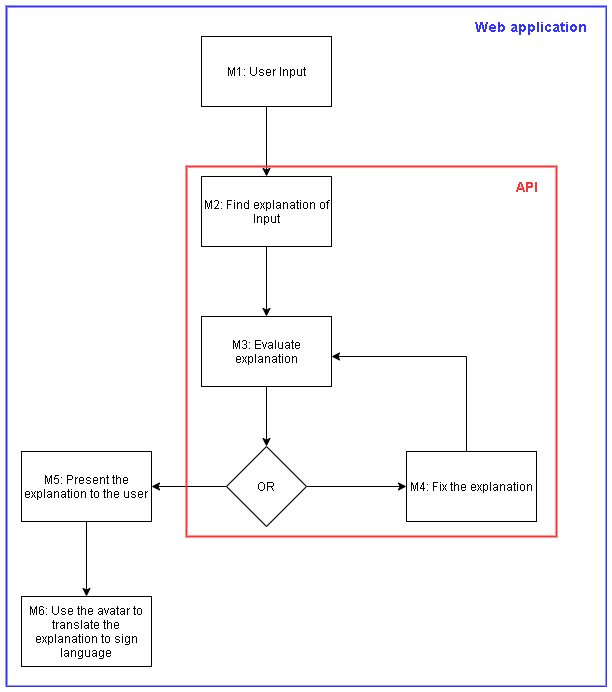
\includegraphics[scale=0.5]{ch4/assets/diagram1_2.png}
\caption[High-Level Approach]{High-Level Approach}
\label{fig:Diagram1}
\end{figure}

In the Figure~\ref{fig:Diagram1} is shown the main build blocks of the web application to be developed.
The input received in M1 is send to the \gls{API} that generates an explanation in M2, which is validated in M3.
From there the explanation might be sent back to the application and shown to the user in M5  or if does not meet all the creteria defined in M3 it will be fixed in M4 and reevaluated.
After presenting the explanation to the user, the application will also be capable of send the text to an already existing \gls{API} that is capable of translate plain text to \gls{PSL} using a avatar in M6.

To help better understand the created design, a more detailed view, is presented below, that describes each of the build blocks and how will they achieve the tasks previously mentioned.

\begin{figure}[H]
\centering
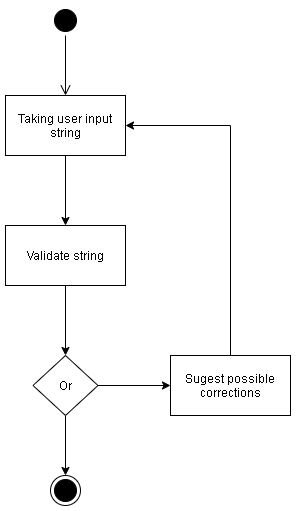
\includegraphics[scale=0.5]{ch4/assets/M1.png}
\caption[User Input Module]{M1: User Input}
\label{fig:M1}
\end{figure}

As shown in the Figure~\ref{fig:M1} the M1 was design to receive a input string from the user.
This string is validated in order to dected common mistakes, such as typos, and when an mistake is detected the application suggests possible corrections.
The user is then capable of accepting the suggestion given, make a manual correction or procede without changing the input string.

\begin{figure}[H]
\centering
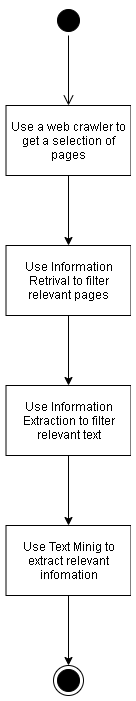
\includegraphics[scale=0.5]{ch4/assets/M2.png}
\caption[Find Explanation Module]{M2: Find Explanation}
\label{fig:M2}
\end{figure}

The Figure~\ref{fig:M2} shows the process of finding an explanation based on the received string.
A web crawler would be use to find all the pages connected to the one \dots

\begin{figure}[H]
\centering
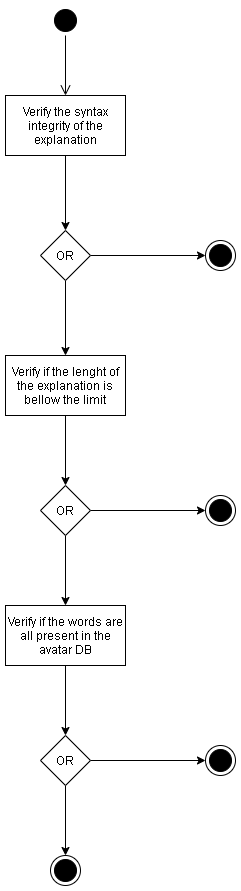
\includegraphics[scale=0.5]{ch4/assets/M3.png}
\caption[Evaluate Explanation Module]{M3: Evaluta Explanation}
\label{fig:M3}
\end{figure}

In Figure~\ref{fig:M3}

\begin{figure}[H]
\centering
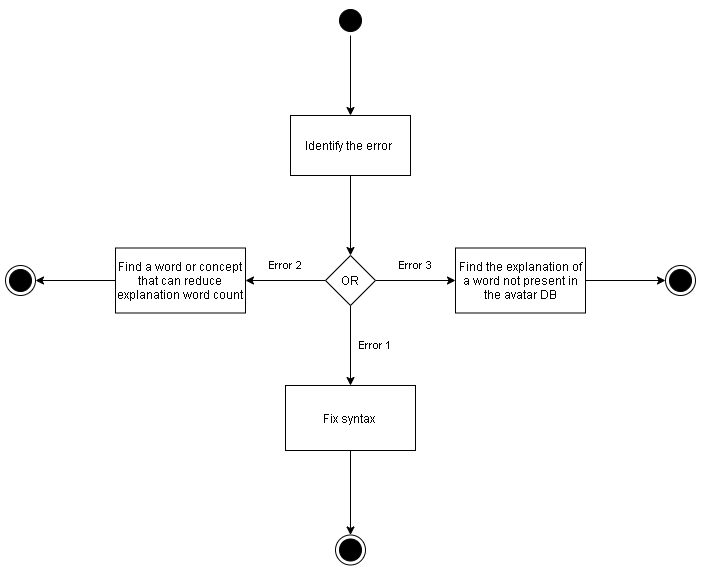
\includegraphics[width=\textwidth,keepaspectratio]{ch4/assets/M4.png}
\caption[Fix Explanation Module]{M4: Fix Explanation}
\label{fig:M4}
\end{figure}

As it can be seen in Figure~\ref{fig:M4}

\begin{figure}[H]
\centering
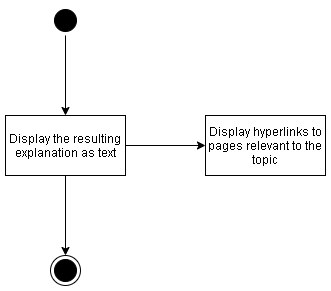
\includegraphics[scale=0.5]{ch4/assets/M5.png}
\caption[Present Explanation Module]{M5: Present Explanation}
\label{fig:M5}
\end{figure}

Figure~\ref{fig:M5}

\begin{figure}[H]
\centering
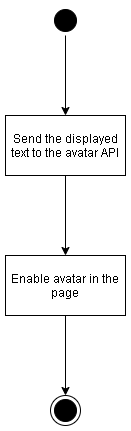
\includegraphics[scale=0.5]{ch4/assets/M6.png}
\caption[Avatar Module]{M6: Avatar}
\label{fig:M6}
\end{figure}

Figure~\ref{fig:M6}


With the complete design of the application in mind a simpler and easier to implement approach was design, also known as a \gls{MVP}.

\begin{figure}[H]
\centering
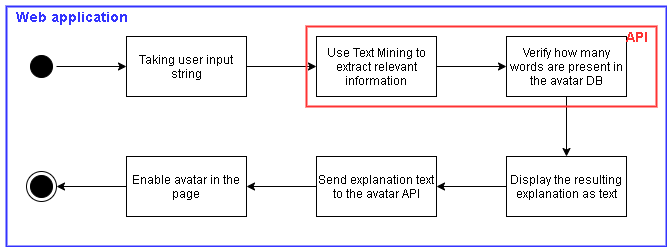
\includegraphics[width=\textwidth,keepaspectratio]{ch4/assets/mvp_2.png}
\caption[Minimun Value Product]{Minimun Value Product}
\label{fig:mvp}
\end{figure}

Figure~\ref{fig:mvp}